\chapter{Resultados}

Este capítulo apresenta os resultados obtidos com a implementação do simulador desenvolvido neste trabalho. São apresentados exemplos de utilização do sistema, demonstrando o funcionamento das funcionalidades implementadas e a correspondência entre o comportamento observado na simulação e a modelagem cinemática descrita nos capítulos anteriores.

\section{Interface do Sistema}

A Figura \ref{fig:interface_completa_final} apresenta a interface principal do simulador desenvolvido. Nela é possível observar a visualização tridimensional do manipulador, os controles de interação e os elementos de análise cinemática disponíveis ao usuário.

\begin{figure}[H]
\centering
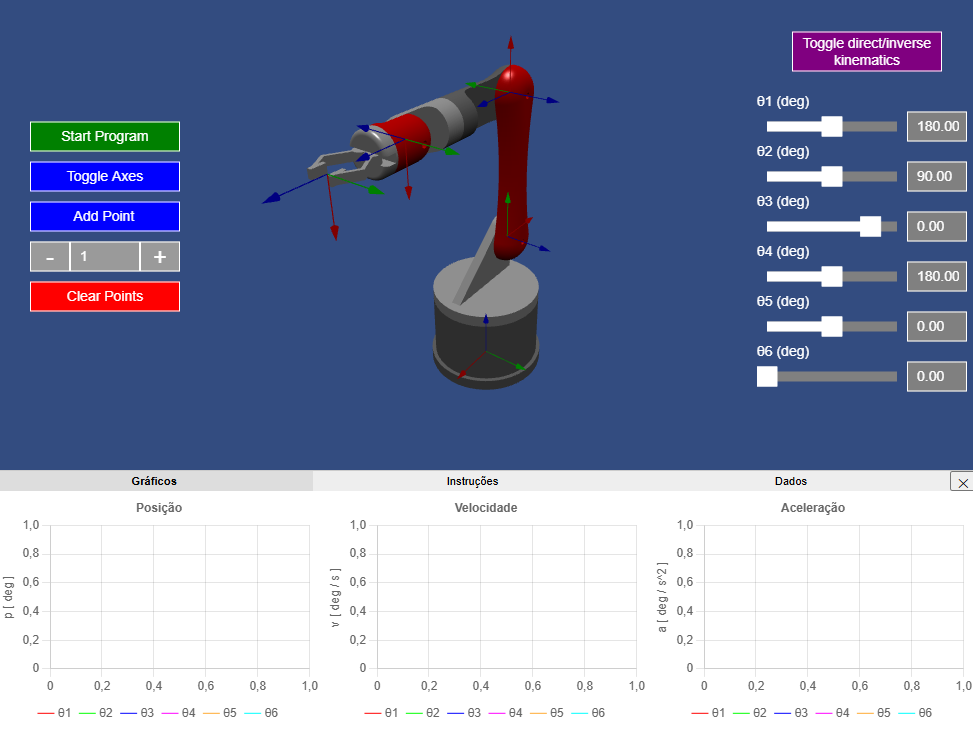
\includegraphics[width=0.8\textwidth]{Imagens/interface_completa_final.png}
\caption{Interface principal do simulador desenvolvido.}
\label{fig:interface_completa_final}
\end{figure}

A interface permite ao usuário interagir diretamente com o manipulador por meio de controles articulares ou cartesianos, além de acompanhar em tempo real os gráficos de posição, velocidade e aceleração das juntas. Também é possível observar a matriz de transformação homogênea do efetuador final e o caminho espacial percorrido durante a execução de trajetórias.

\section{Testes de Cinemática Direta}

Para verificar o funcionamento da cinemática direta implementada no simulador, foram realizados testes utilizando diferentes configurações articulares. Em cada caso, os valores das variáveis articulares foram definidos manualmente por meio dos controles deslizantes da interface, permitindo observar a configuração espacial resultante do manipulador.

A Figura \ref{fig:teste_cd} apresenta um exemplo de configuração articular aplicada ao manipulador. Na interface também são exibidos a matriz de transformação homogênea global do efetuador final, a tabela de parâmetros de Denavit--Hartenberg e os eixos locais associados às juntas.

\begin{figure}[H]
\centering
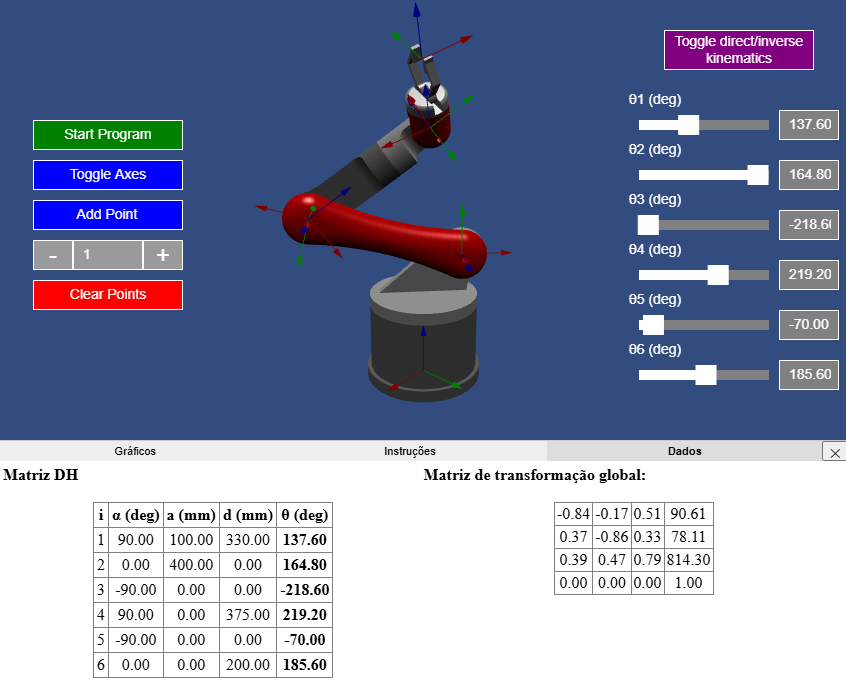
\includegraphics[width=0.9\textwidth]{Imagens/teste_cinematica_direta.png}
\caption{Exemplo de configuração do manipulador obtida a partir de valores específicos das variáveis articulares.}
\label{fig:teste_cd}
\end{figure}

A partir dessa configuração, o simulador calcula automaticamente a matriz de transformação homogênea do efetuador final, exibida na interface. O resultado obtido é consistente com a modelagem baseada na Convenção de Denavit–Hartenberg apresentada no Capítulo 2.

\section{Testes de Cinemática Inversa}

A validação da implementação da cinemática inversa foi realizada por meio da comparação entre a pose cartesiana definida pelo usuário e a matriz de transformação homogênea resultante exibida pelo simulador.

No modo de controle cartesiano, o usuário define diretamente a posição do efetuador final por meio das coordenadas $x$, $y$ e $z$, bem como sua orientação utilizando os ângulos \textit{roll}, \textit{pitch} e \textit{yaw}. A partir desses valores, o algoritmo de cinemática inversa calcula automaticamente o conjunto correspondente de variáveis articulares, que são então aplicadas ao manipulador.

A Figura \ref{fig:teste_ci} apresenta um exemplo de pose definida pelo usuário utilizando os controles cartesianos da interface.

\begin{figure}[H]
\centering
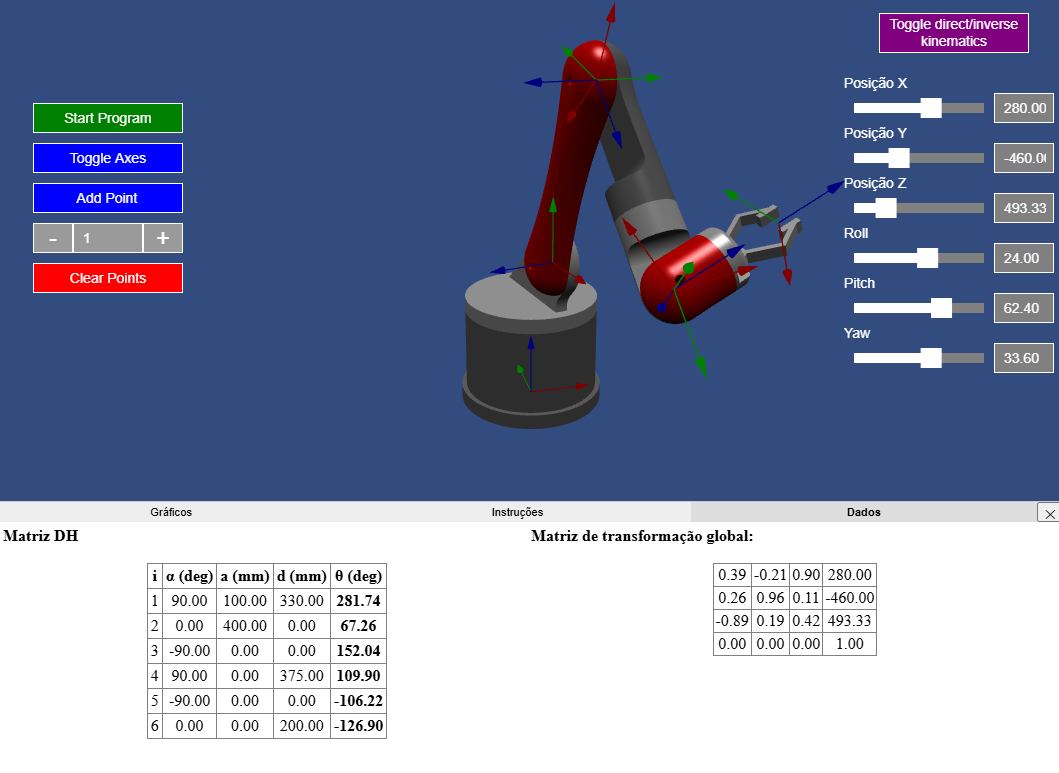
\includegraphics[width=0.9\textwidth]{Imagens/teste_ci.png}
\caption{Exemplo de validação da cinemática inversa a partir de uma pose cartesiana especificada pelo usuário.}
\label{fig:teste_ci}
\end{figure}

No exemplo apresentado, o usuário definiu a posição do efetuador final como:

\begin{align}
x &= 280.00 \\
y &= -460.00 \\
z &= 493.33
\end{align}

Após a execução da cinemática inversa, o simulador calcula as variáveis articulares correspondentes e atualiza a matriz de transformação homogênea global do efetuador final, exibida na interface na forma:

\begin{equation}
^0T_6 =
\begin{bmatrix}
0.39 & -0.21 & 0.90 & 280.00 \\
0.26 & 0.96 & 0.11 & -460.00 \\
-0.89 & 0.19 & 0.42 & 493.33 \\
0 & 0 & 0 & 1
\end{bmatrix}
\end{equation}

A validação da solução pode ser realizada diretamente a partir da estrutura dessa matriz. Conforme apresentado no Capítulo 2, a última coluna da matriz de transformação homogênea corresponde ao vetor posição do efetuador final:

\begin{equation}
p =
\begin{bmatrix}
x \\
y \\
z
\end{bmatrix}
\end{equation}

Observa-se que os valores da última coluna da matriz calculada coincidem exatamente com os valores definidos pelo usuário nos controles deslizantes de posição, confirmando a consistência da solução obtida para a posição do efetuador.

Em seguida, pode-se validar a orientação do efetuador final a partir dos ângulos definidos pelo usuário. No exemplo da Figura \ref{fig:teste_ci}, foram especificados os valores:

\begin{align}
\text{roll} &= 24.00^\circ \\
\text{pitch} &= 62.40^\circ \\
\text{yaw} &= 33.60^\circ
\end{align}

No simulador, esses ângulos são utilizados para compor a matriz de rotação do efetuador segundo a convenção ZYX, dada por:

\begin{equation}
R = R_z(\text{yaw})\,R_y(\text{pitch})\,R_x(\text{roll})
\end{equation}

com

\begin{equation}
R =
\begin{bmatrix}
c_y c_p & c_y s_p s_r - s_y c_r & c_y s_p c_r + s_y s_r \\
s_y c_p & s_y s_p s_r + c_y c_r & s_y s_p c_r - c_y s_r \\
-s_p    & c_p s_r               & c_p c_r
\end{bmatrix}
\end{equation}

onde, por simplicidade, adotou-se a notação:

\[
c_y = \cos(\text{yaw}), \quad s_y = \sin(\text{yaw}),
\]
\[
c_p = \cos(\text{pitch}), \quad s_p = \sin(\text{pitch}),
\]
\[
c_r = \cos(\text{roll}), \quad s_r = \sin(\text{roll})
\]

Substituindo os valores definidos no exemplo, obtém-se:

\begin{equation}
R =
\begin{bmatrix}
0.39 & -0.21 & 0.90 \\
0.26 & 0.96 & 0.11 \\
-0.89 & 0.19 & 0.42
\end{bmatrix}
\end{equation}

Esse resultado coincide com a submatriz de rotação correspondente às três primeiras colunas e três primeiras linhas da matriz de transformação homogênea exibida na interface do simulador. Dessa forma, confirma-se que a orientação especificada pelos controles \textit{roll}, \textit{pitch} e \textit{yaw} está corretamente refletida na pose final calculada pelo sistema.

\section{Execução de Trajetórias}

O simulador permite a execução de trajetórias definidas a partir de uma sequência de configurações articulares intermediárias. Para avaliar essa funcionalidade, foram programados diferentes movimentos utilizando a interpolação polinomial cúbica descrita anteriormente.

A Figura \ref{fig:trajetoria_execucao} apresenta um exemplo de execução de trajetória no simulador.

\begin{figure}[H]
\centering

\includegraphics[width=0.8\textwidth]{Imagens/planejamento_trajetoria.png}
\caption{Execução de trajetória programada no simulador.}
\label{fig:trajetoria_execucao}
\end{figure}

Durante a execução do movimento, o sistema atualiza continuamente a posição das juntas e registra o caminho percorrido pelo efetuador final no espaço tridimensional.

\section{Análise dos Gráficos Gerados}

Durante a execução das trajetórias programadas, o simulador gera automaticamente gráficos correspondentes às variáveis de posição, velocidade e aceleração das juntas.

A Figura \ref{fig:grafico_trajetoria} apresenta os gráficos gerados após a execução do movimento programado exibido na Figura \ref{fig:trajetoria_execucao}

\begin{figure}[H]
\centering
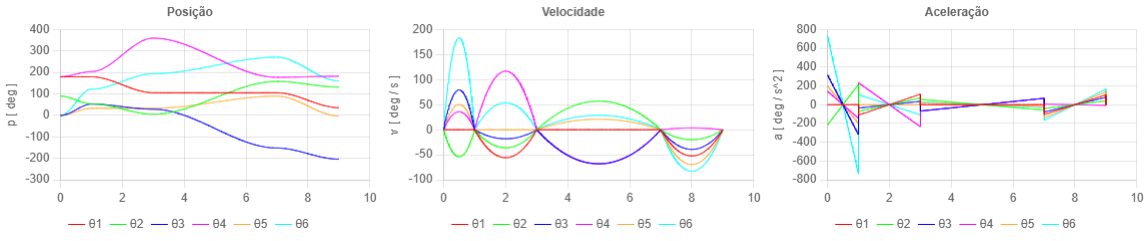
\includegraphics[width=1\textwidth]{Imagens/graficos_exemplo.png}
\caption{Perfis de posição, velocidade e aceleração gerados durante a execução de uma trajetória.}
\label{fig:grafico_trajetoria}
\end{figure}

Observa-se que os perfis apresentam comportamento suave e contínuo, conforme esperado para trajetórias geradas por interpolação polinomial cúbica. A continuidade das curvas confirma o correto funcionamento da implementação descrita no Capítulo 3.

\section{Discussão dos Resultados}

Os resultados obtidos demonstram que o simulador é capaz de reproduzir de forma consistente os principais conceitos da cinemática de manipuladores robóticos. As funcionalidades implementadas permitem explorar tanto o espaço das juntas quanto o espaço cartesiano, além de visualizar em tempo real as transformações geométricas associadas ao movimento do manipulador.

A integração entre visualização tridimensional, representação matricial e gráficos cinemáticos contribui para tornar mais intuitiva a compreensão dos conceitos abordados nas disciplinas de automação e robótica.

Dessa forma, a ferramenta desenvolvida apresenta potencial como recurso de apoio didático para o ensino de cinemática de manipuladores, permitindo que os estudantes experimentem interativamente diferentes configurações e observem seus efeitos sobre o movimento do robô.